\section{Umelá inteligencia}\label{sec:ai}

Od počiatku vzniku mechanických strojov, ktoré pomáhajú ľuďom pri svojej práci sa pri nich nepriamo niesol aj pojem
\enquote{umelá inteligencia}.
Medzi odbornou verejnosťou tento pojem stále nie je jednotný, no väčšina z nich má rovnakú myšlienku:
inteligencia vykonávaná strojmi (narozdiel od prirodzenej inteligencie, ktorú vykonávajú ľudia, či
zvieratá).\cite{ai_definition}
Ak stroj (aj mechanický) dokáže niečo vykonať bez explicitného príkazu, je považovaný za inteligentný.

\subsection{Metódy}\label{subsec:ai-methods}

Umelá inteligencia (angl. artificial intelligence) je široká vedná disciplína, ktorá zahŕňa
\begin{itemize}
    \item strojové učenie
    \item textovú analýza
    \item analýzu reči
    \item prevod textu na reč
    \item expertné systémy
    \item plánovanie
    \item optimalizáciu
    \item robotiku
    \item analýzu obrazu
    \item a mnoho ďalšieho
\end{itemize}
Metódy niektorých skupín sa môžu prelínať (napr. na analýzu obrazu a na analýzu zvuku sa môžu použiť umelé neurónové
siete).\cite{ai_ann_sound,ai_ann_image}
Dôsledkom toho je aj fakt, že niektoré metódy sa používajú viac a iné menej.
Využiteľnosť metód závisí teda najmä od problému, ktorý riešia.

Ak problémom je plánovanie trasy pre kuriérov, použije sa matematická optimalizácia.
Ukážkou môže byť ako americká spoločnosť UPS v amerických mestách, kde je systém ulíc riešený kolmým spôsobom, čo
najviac obmedzila zatáčanie kuriérov \emph{vľavo}.\cite{ups_optimization}
Dôvodom je najmä to, že keď kuriér odbočuje vľavo, musí dať prednosť protiidúcim vozidlám, pričom auto stojí na
križovatke naštartované.
Dôsledkom sú nasledovné vylepšenia:
\begin{enumerate}
    \item ušetrených takmer 40 miliónov litrov paliva ročne
    \item o 100 tisíc ton $CO_2$ menej
\end{enumerate}
Rovnaké vylepšenia by prinieslo odstavenie 21 tisíc áut.

Na druhú stranu, keď sa rieši problém rozpoznávania hlasových príkazov je nutné problém rozdeliť na 2 podproblémy:
\begin{enumerate}
    \item \emph{spracovanie zvuku}, napr. s využitím skrytých markovových modelov\cite{hmm}
    \item \emph{spracovanie textu}\cite{text_analysis}
\end{enumerate}

Je teda zjavné, že algoritmus, ktorý rozpoznáva význam textu nebude stačiť pre plánovanie trás kuriérov.
Nižšie sú popísané metódy, ktoré sú v rámcu umelej inteligencie využívané najlepšie.

\subsubsection{Heuristické metódy}

Heuristiky sú často používanou metódou vo vyhľadávacích algoritmoch.\cite{heuristic}
Na rozdiel od exaktných algoritmov, ktoré prehľadávajú celý vyhľadávací priestor, heuristiky prehľadávajú len okolie
východiskového riešenia.
Ak napríklad je cieľom heuristiky nájsť minimum nejakej funkcie (nemusí byť zadaná analyticky) v $n$-rozmernom priestore,
dokáže táto metóda nájsť len lokálne minimum závislé na tom, kde sa nachádza východzie riešenie.
Príklad je uvedený pre funkciu
\begin{equation}
    f(x,y)=e^{\cos(x)+\sin(y)}\frac{x+y}{30}+\frac{5}{2}
\end{equation}
kde $x\in<-12,12>$, $y\in<-12,12>$.
\begin{figure}[H]
    \centering
    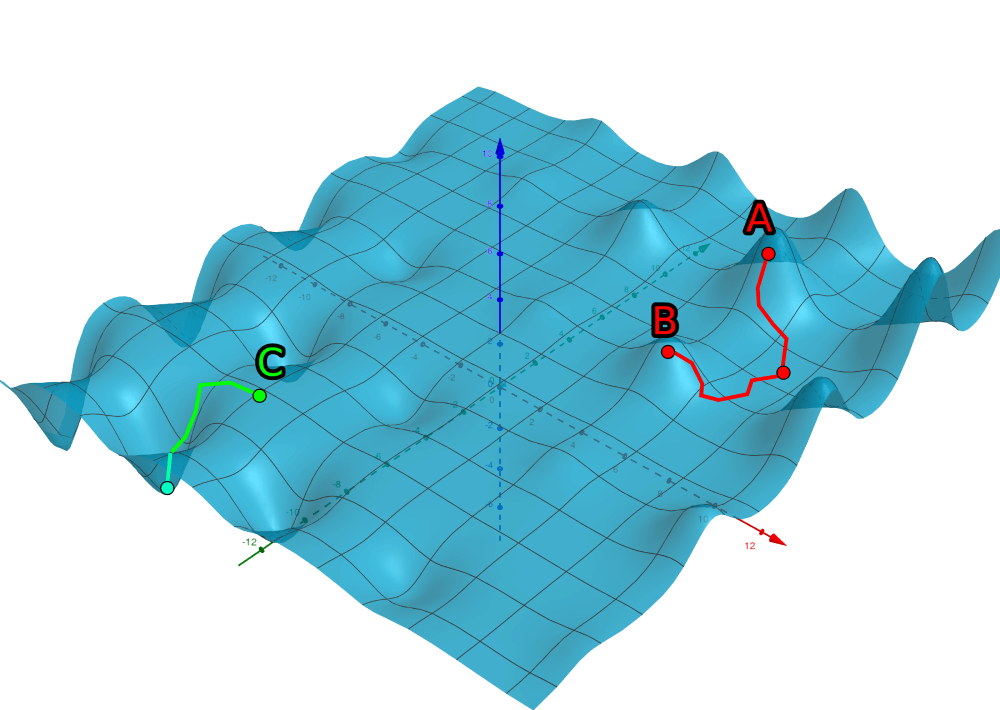
\includegraphics[width=0.8\textwidth]{images/heuristic.png}
    \caption{Heuristika a jej riešenia v závislosti od východzieho riešenia}
\end{figure}\label{figure:heuristic-method}
Pri nastavení východiskového bodu \textbf{A} alebo \textbf{B} nájde heuristika rovnaké lokálne minimum (čo sa môže javiť
ako globálne), no pre východzí bod \textbf{C} nájde algoritmus globálne minimum, čo ale nie je možné overiť bez
prehľadania celého priestoru riešení.
Z toho je možné usúdiť, že riešenie heuristiky nie je vždy optimálne a nikdy jeho optimálnosť nie je zaručená, ale na
druhú stranu sú heuristiky extrémne rýchle.
Heuristické metódy patria medzi najzákladnejšie techniky v rámci umelej inteligencie.

Ako ukážkový príklad praktického využitia heuristických metód je možné uviesť hľadanie najkratšej (alebo najrýchlejšej)
cesty medzi dvoma mestami v cestnej sieti Slovenska pre navigačné systémy alebo pohyb neovládaných postáv v hrách
(angl. non-player character, skr. NPC - akákoľvek postava v hre, ktorú neovláda človek).
Pre oba tieto príklady je možné použiť napríklad \emph{A* algoritmus}.\cite{heuristic}

\subsubsection{Metóda podporných vektorov}

Anglicky support vector machine (skr. SVM) je metóda strojového učenia s učiteľom (reinforcement
learning).\cite{support_vector_machine}
Cieľom tejto metódy je nájsť takú \emph{nadrovinu} v $n$-rozmernom vyhľadávacom priestore, ktorá vstupné dáta rozdelí
do dvoch podpriestorov.
Metóda je určená pre klasifikáciu a regresnú analýzu.
Ak je metóda konštruovaná ako optimalizačná úloha jej účelová funkcia vyzerá podobne ako nasledovná:
\begin{equation}
    \max \sum_{\forall i}{\sqrt{\sum_{\forall j}{(\vec{v}_j - x_{ij})^2}}}
\end{equation}
Kde $\vec{v}$ je hľadaný vektor a $\vec{v}_j$ sú jeho zložky a kde $x_i$ je vzorka zo vstupných dát a $x_{ij}$ sú jeho
zložky.
Keďže výraz $\sqrt{\sum_{\forall j}{(\vec{v}_j - x_{ij})^2}}$ vyjadruje najmenšiu vzdialenosť medzi vektorom a
vzorkou, dá sa povedať, že metóda hľadá takú nadrovinu, ktorá vyhľadávací priestor rozdelí čo najlepšie.
\begin{figure}[H]
    \centering
    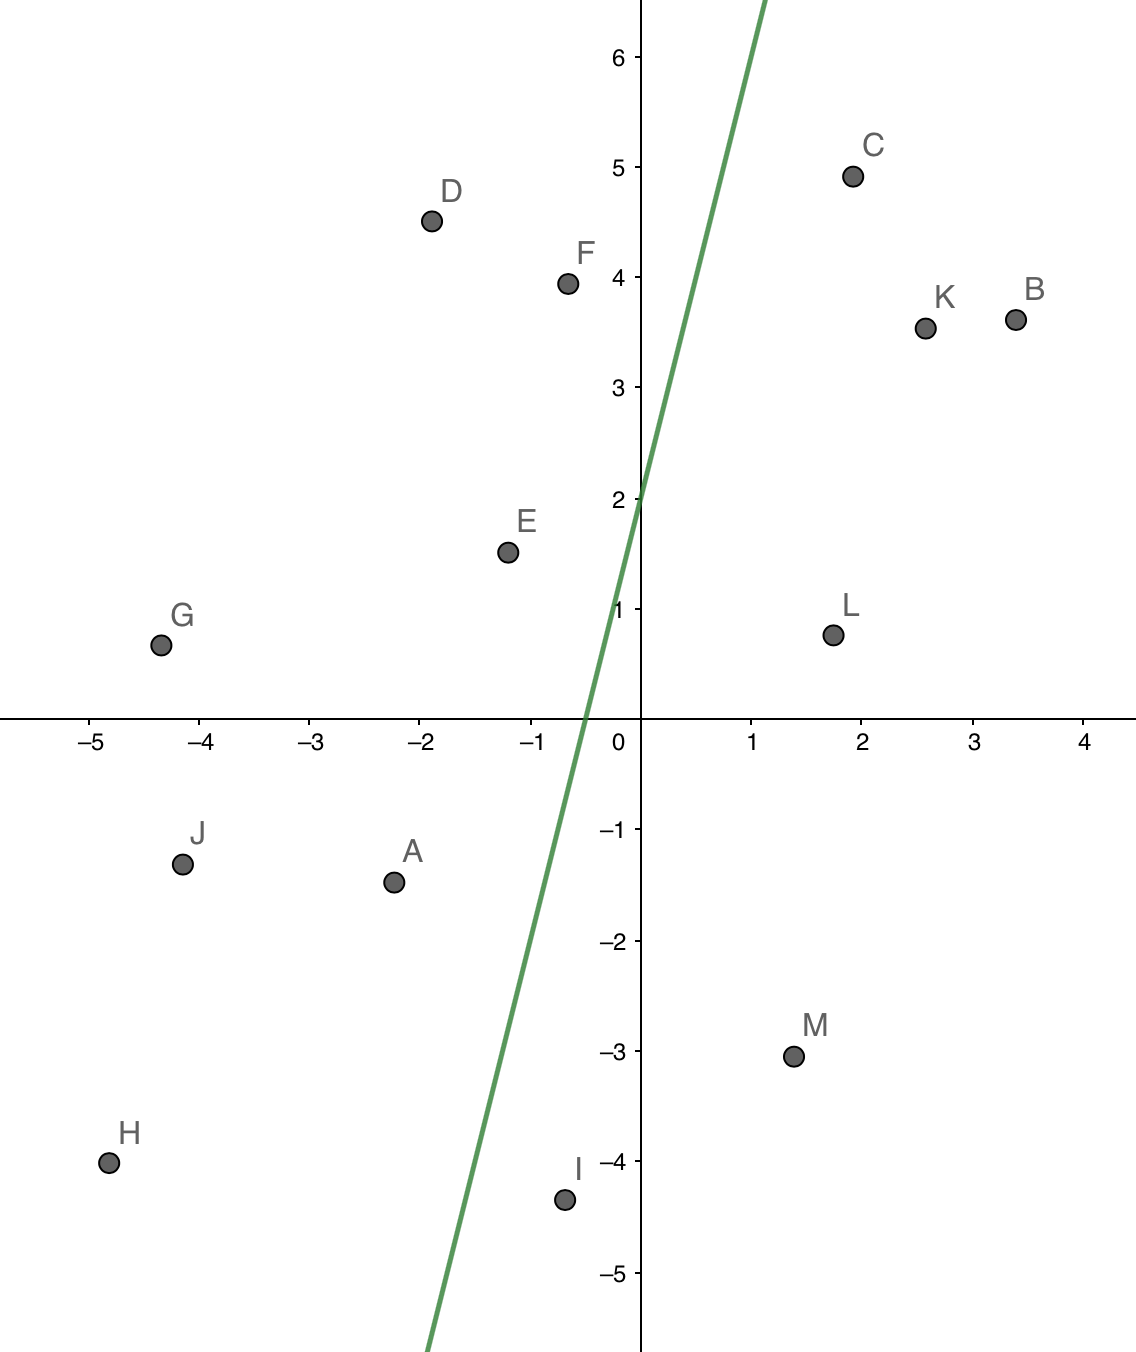
\includegraphics[width=0.5\textwidth]{images/svm.png}
    \caption{Support vector machine}
\end{figure}\label{figure:svm}

Typickým príkladom použitia metódy podporných vektorov je rozdelenie e-mailovej komunikácie do dvoch skupín: relevantnú
a nevyžiadanú poštu, no podporné vektory sa dajú použiť aj na spracovanie obrazu, či textu.

\subsubsection{Iné metódy}

Pre umelú inteligenciu existuje veľké množstvo algoritmov a ich alternatív, z ktorých sú ešte často používané
\emph{umelé neurónové siete}, ktoré sú bližšie popísané v \autoref{subsec:algo-ann} a ako rozhodovacie pravidlo v
teórii hier je často využívaný algoritmus \emph{minimax} (viac v \autoref{subsec:algo-minmax}).
